

\chapter{Einführung}



Das übergeordnete Ziel des hier vorgestellten Studienprojektes ist es ein Fahrzeug autonom einen Raum erkunden zu lassen. Dabei soll eine vollständige Karte des Raumes mit der Hilfe des \acrfull{slam} Algorithmus erstellt und visualisiert werden. Durch den Einsatz verschiedener integrierter Sensoren am \textit{ALF} soll diese autonome Navigation umgesetzt werden. 
Auf eine externe Steuerung wird verzichtet, da der Fokus auf die autonome Erkundung gelegt wurde. Die Arbeit sollte auf der Hardware und Software vorheriger Gruppenarbeiten aufgesetzt werden. Zum Projektstart waren aber bereits sehr viele Probleme vorhanden, deswegen wurde sich für einen neuen verbesserten Aufbau in Hard- und Software entschieden. In den nachfolgenden Kapiteln erfolgt eine ausführliche Dokumentation der Umsetzung.


%\vspace{0.1cm}
\begin{figure}[hbtp]
\centering
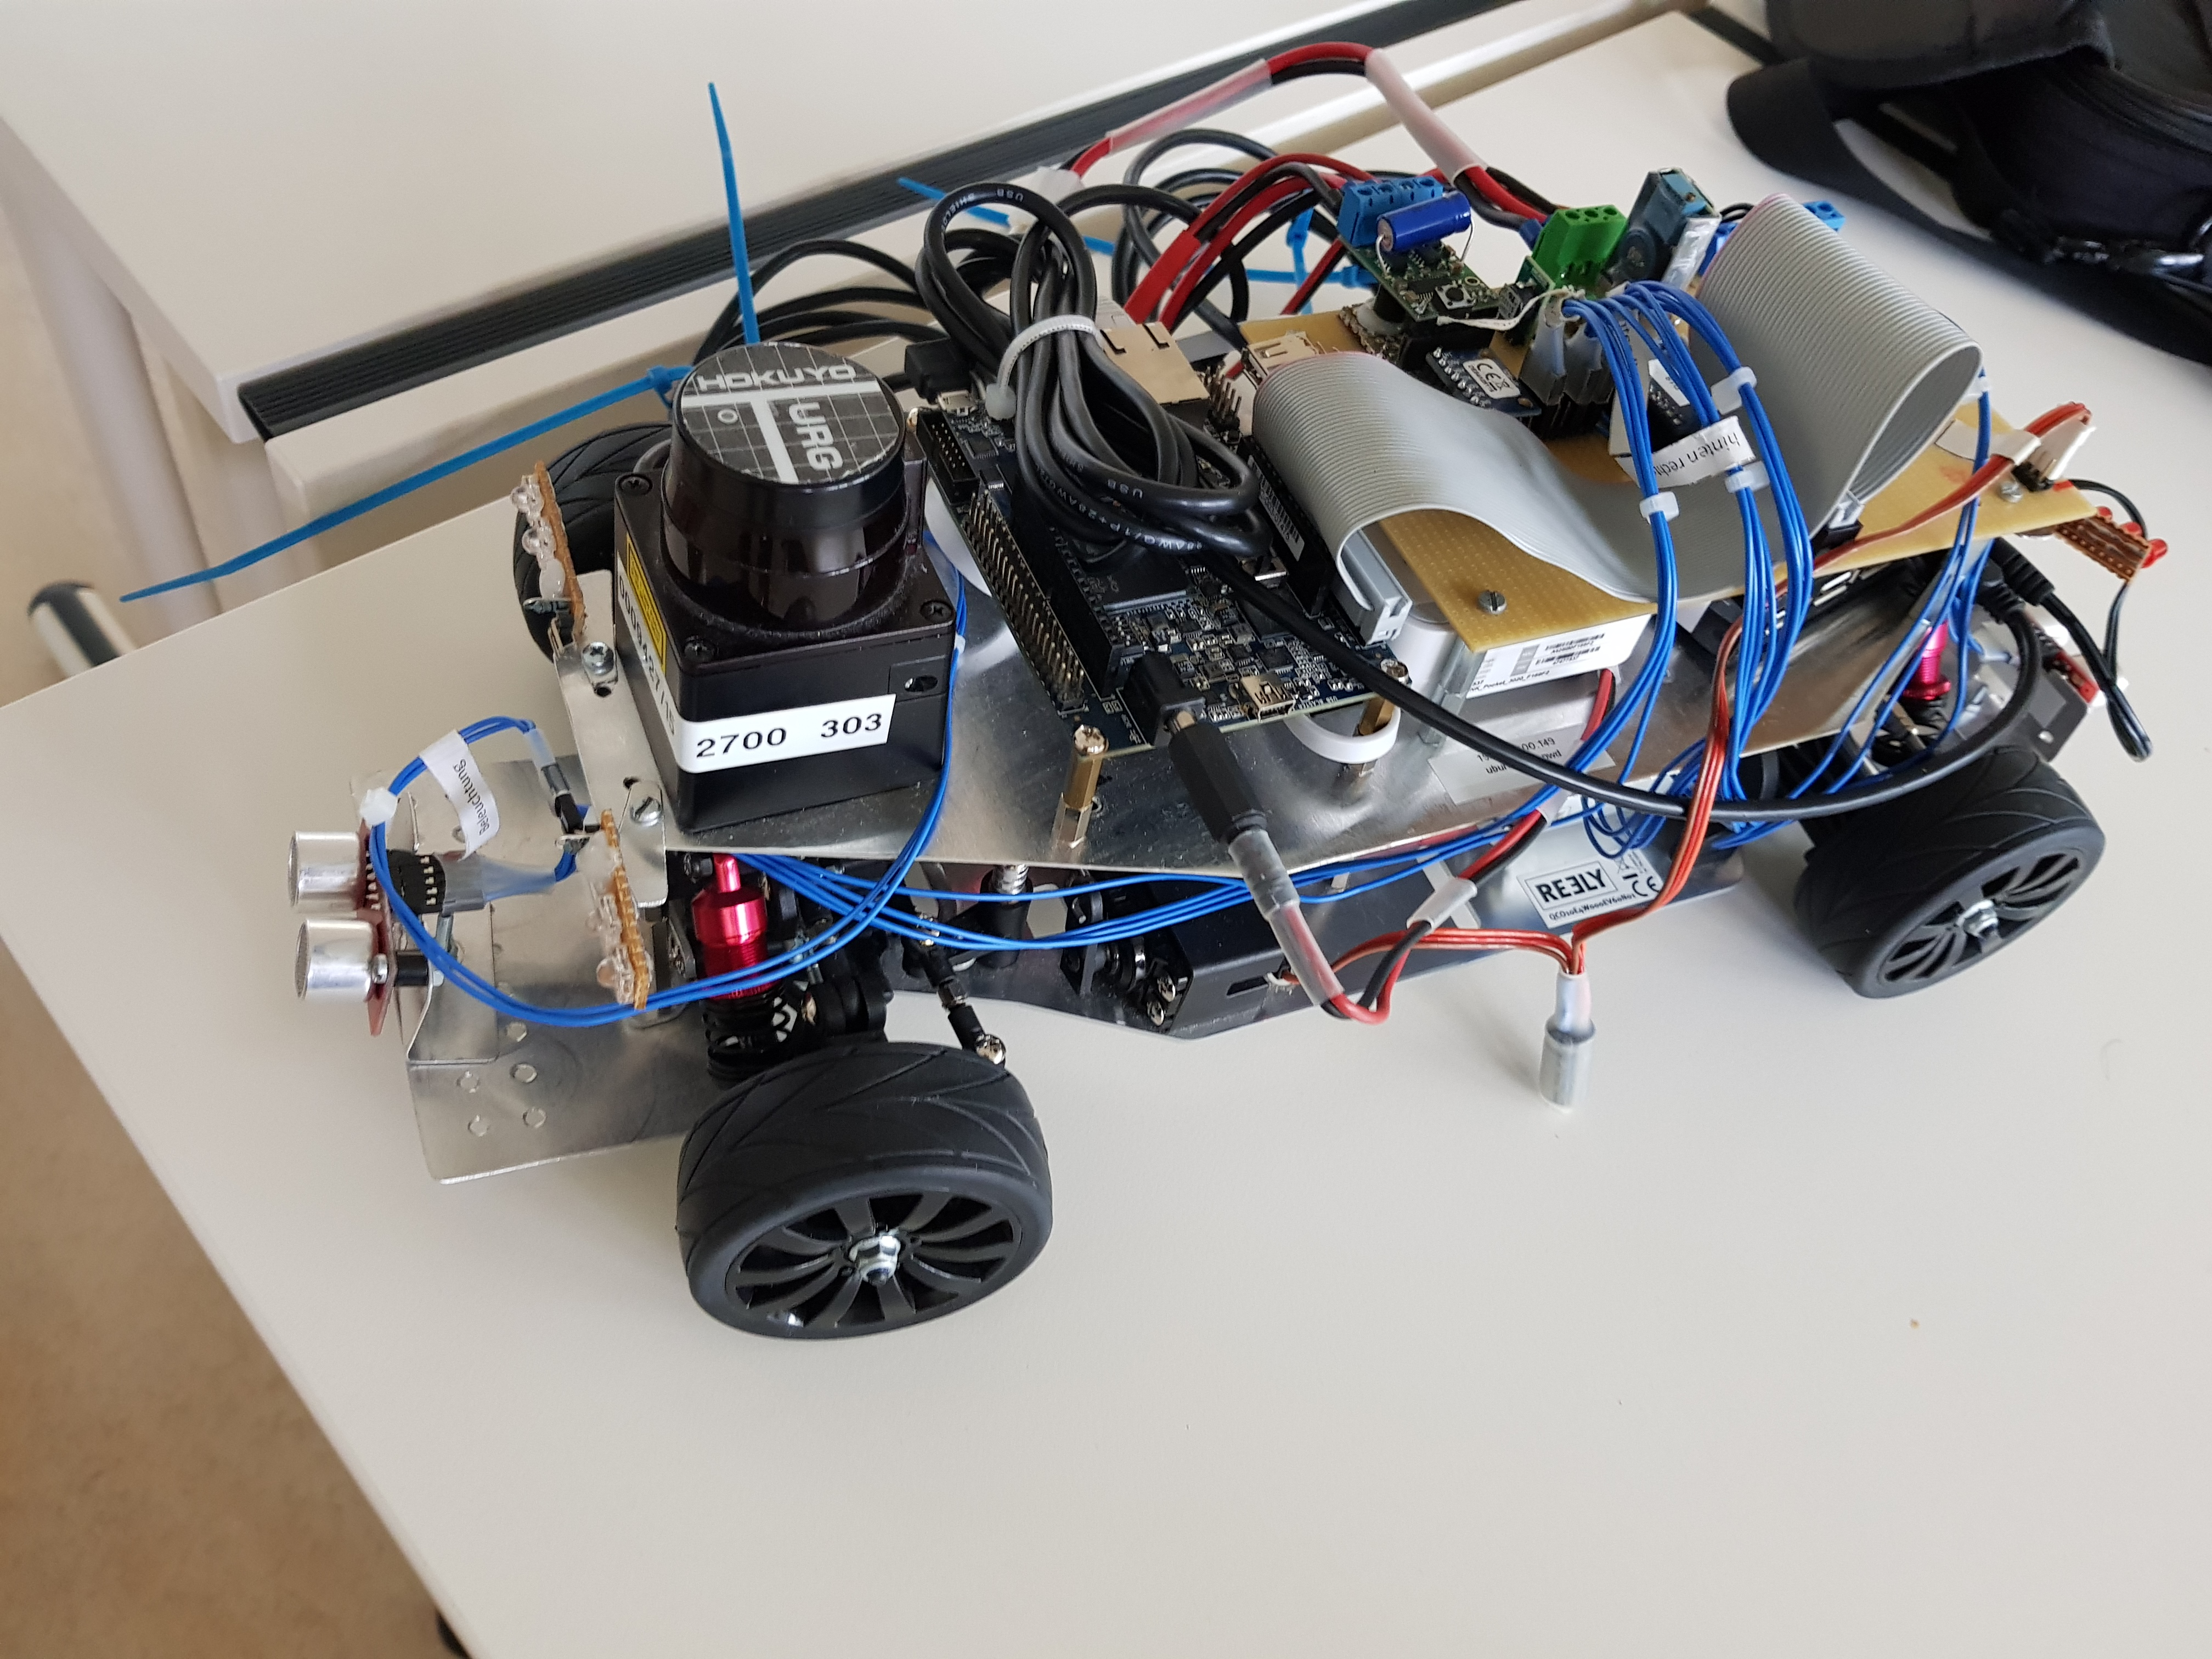
\includegraphics[scale=0.105]{images/chapter2/alf_old.jpg}
\caption{Aufbau des ALF zu Beginn des Projektes}
\label{fig:alf_old}
\end{figure}